\documentclass{article}
\usepackage[T1]{fontenc}
\usepackage{iclr2027_conference,times}
\usepackage{amsmath,amssymb,amsthm,mathtools}
\usepackage{graphicx,booktabs,array,multirow}
\usepackage{wrapfig,placeins,pifont}
\usepackage{microtype,xcolor,url,hyperref}
\usepackage{tikz}
\usetikzlibrary{positioning,arrows.meta,fit,backgrounds,calc}

\definecolor{dsblue}{HTML}{2A78D6}
\definecolor{dsorange}{HTML}{EB6834}
\definecolor{dsgray}{HTML}{8A8984}
\newcommand{\parahead}[1]{\paragraph{#1}}

\hypersetup{colorlinks=true,linkcolor=black,citecolor=black,urlcolor=black,
  pdftitle={Expert Parallelism on a Laptop: Running a 754B-Parameter MoE in 24 GB},
  pdfauthor={Haorui Li}}
\title{Expert Parallelism on a Laptop:\\Running a 754B-Parameter MoE in 24\,GB}
\author{%
\textbf{Haorui Li}\\
Southeast University\\
\href{mailto:haoruileee@gmail.com}{\texttt{haoruileee@gmail.com}}
}
\iclrfinalcopy % Non-anonymous preprint.
\makeatletter
\renewcommand{\@maketitle}{\vbox{\hsize\textwidth\centering
  \def\@makefnmark{\hbox{\@textsuperscript{\normalfont\@thefnmark}}}%
  {\LARGE\scshape\@title\par}
  \def\And{\end{tabular}\hspace{2em}%
    \begin{tabular}[t]{c}\rule{\z@}{24pt}\ignorespaces}%
  \begin{tabular}[t]{c}\rule{\z@}{24pt}\@author\end{tabular}\par
  \vskip 0.6em
  {\normalfont\small\url{https://github.com/haoruilee/DeepInfer-Mac}\par}
  \vskip 0.3in minus 0.1in
}}
\makeatother
\newcommand{\method}{\textsc{DeepInfer-Mac}}
\newcommand{\relu}[1]{\left[#1\right]_{+}}
\newcommand{\norm}[1]{\left\lVert#1\right\rVert_2}
\newcommand{\topk}{\operatorname{TopK}}
\newcommand{\bfround}{\operatorname{bf16}}
\newcommand{\q}{\mathbf q}
\newcommand{\kv}{\mathbf k}
\newcommand{\RR}{\mathbb R}
\newtheorem{proposition}{Proposition}
\newtheorem{lemma}{Lemma}
\begin{document}
\maketitle
\lhead{} % No conference publication or review header in the preprint.
\begin{abstract}
DeepSeek serves its 754B-parameter DeepSeek-V4.1-Flash model with expert parallelism. The experts of each layer are spread over many GPUs, every token is sent to the GPUs that hold its experts, and communication is hidden behind computation. We ask what remains of this design on a single laptop with 24\,GB of memory. Our system, \method{}, keeps the dense weights in memory and leaves the experts on the internal SSD. After routing, it reads each missing expert straight into a preallocated GPU buffer. Decoding a token then becomes a chain in which the router must finish before the reads can start, and the next layer must wait for the experts. The SSD therefore sits idle while the GPU works, and the cluster's overlap techniques recover little of that time. Prefetching the next layer's experts even makes decode slower, because the guesses delay the reads the token is waiting for. We fix this with idle-window speculation, which issues the guesses only after the current layer's reads have landed. This simple change makes decode 11--27\% faster across all cache sizes we tested and leaves the output unchanged. On a MacBook Air, \method{} decodes 1.23 tokens per second while keeping 9\,GB free for macOS, and it stays close to DeepSeek's own deployment on open-ended text. We also show that the model's sparse-attention indexer can use BF16 matrix units without changing its scores, which roughly halves its cost in long prefill.
\end{abstract}

\section{Introduction}
Mixture-of-experts (MoE) models activate only a small part of their parameters for each token \citep{switch,deepseekv3}. DeepSeek-V4.1-Flash has 754B parameters in 40 layers, and each layer has 384 routed experts, of which a token uses six \citep{deepseek41flash}. In the data center, DeepSeek serves this model with expert parallelism (EP) \citep{deepinfer}. The experts of a layer are spread over many GPUs, and after routing each token is sent to the GPUs that hold its experts. The cost of this communication is hidden by overlapping two micro-batches, and frequently used experts are replicated.

This paper asks whether the same model can run on a MacBook Air with 24\,GB of memory, and which of these techniques still help there. The converted model takes 338\,GB, so it cannot be held in memory. However, the work for one token is much smaller. The dense layers take 7.6\,GB at 8 bits per weight, and the six experts per layer that a token needs take about 3.3\,GB in total. The laptop also has a second device that can store experts: an SSD that reads about 3\,GB/s. We therefore treat the SSD as the expert-holding device, the role that other GPUs play under EP.

We built \method{} around this idea (Figure~\ref{fig:overview}). After routing, the engine reads each missing expert from the SSD with one \texttt{preadv} call directly into a slot of a GPU buffer, without copies and without the OS page cache, and runs all experts of the layer in one gathered quantized matmul. Recently used experts stay in memory as a cache, which plays the role of expert replication.

Measuring this system showed where the time goes. A decoding token forms a strict chain in every layer: the router decides which experts to read only after attention, and the next layer can start only after the experts are computed. The SSD is therefore idle while the GPU works, and the GPU waits while the SSD reads. The cluster's micro-batch overlap helps little here: computing the cached experts while the missing ones load made decode 5\% faster. Prefetching the next layer's experts \citep{moeoffload} should fill the idle time, but in our measurements it made decode 5--11\% slower. An interleaved ablation shows why: the guesses compete with reads the token is waiting for. \emph{Idle-window speculation} issues the guesses only after the current layer's misses have arrived, so that they use the SSD while the GPU computes; it also inserts them at the cold end of the cache, which adds a small gain within our confidence intervals. This makes decode 11--27\% faster at every cache size we tested and leaves the output unchanged. In three traced tokens per setting, the SSD is busy 62--65\% of a decode step without speculation and 73--89\% with it.

The engine follows the official reference implementation op by op. It includes compressed sparse attention, Engram memory, Hyper-Connections \citep{hyperconnections}, the vision encoder, DSpark drafting and the FP8/FP4 roundings used in training, and our tests run the official PyTorch model as an oracle.

In summary, we make the following contributions:
\begin{itemize}
  \item \textbf{Expert parallelism on one laptop.} We map EP to one GPU and one SSD: experts move to the GPU through zero-copy reads into fixed buffer slots, and an LRU cache replaces expert replication. We are not aware of another system that runs every component of DeepSeek-V4.1-Flash, including Engram, Hyper-Connections and vision, within 24\,GB with parity tests against the reference (Sections~\ref{sec:design} and~\ref{sec:impl}).
  \item \textbf{A cost model and a study of parallelism.} We model a decode step as a chain of compute and SSD reads. A two-parameter fit matches measured decode speed within 2\% across cache sizes; applied to the speculation runs it shows that speculative reads are not free, and traces show that they mostly fill time when the SSD was idle. We test parallelism at six levels and find which kinds help: those that give the SSD work while the chain leaves it idle, without taking memory or bandwidth from demand reads (Sections~\ref{sec:chain} and~\ref{sec:parallel-eval}).
  \item \textbf{Idle-window speculation.} We find why next-layer expert prefetching \citep{moeoffload} slows decode on a memory-bound laptop: the guesses delay reads the token is waiting for. Issuing guesses only after the demand reads have landed, a known prefetch-control idea, turns the slowdown into a speed-up; an ablation separates it from cold insertion, which adds little (Section~\ref{sec:spec} and~\ref{sec:parallel-eval}).
  \item \textbf{An exactly equal, faster indexer.} We prove that, when the scales of each FP4 block product differ by at most $2^9$ the products stay in the normal FP32 range and the matrix units accumulate in FP32, the FP32 indexer score of DSA-style indexers can be computed with BF16 matrix units without changing a bit. Together with a fused head reduction, this makes the indexer about $2\times$ faster in long prefill ($1.8$--$2.1\times$ on three layers, $3.5\times$ on one). We also measure DoSA's exact screening \citep{dosa} on this model's compressed two-level indexer, where it saves little at 16--32K keys (Section~\ref{sec:indexer}).
\end{itemize}
On a MacBook Air (M4, 24\,GB), \method{} decodes 1.23 tokens/s with a 5.5\,GB expert cache, which keeps 9\,GB free for macOS, and 1.35 tokens/s with 6.5\,GB. Its next-token predictions agree with DeepSeek's API on 86.0\% of open-ended continuation tokens, and it answers a retrieval question correctly at every tested length up to 16K tokens. The code, converter, tests and measurement scripts are open source.

\begin{figure}[t]
\centering
\resizebox{\linewidth}{!}{%
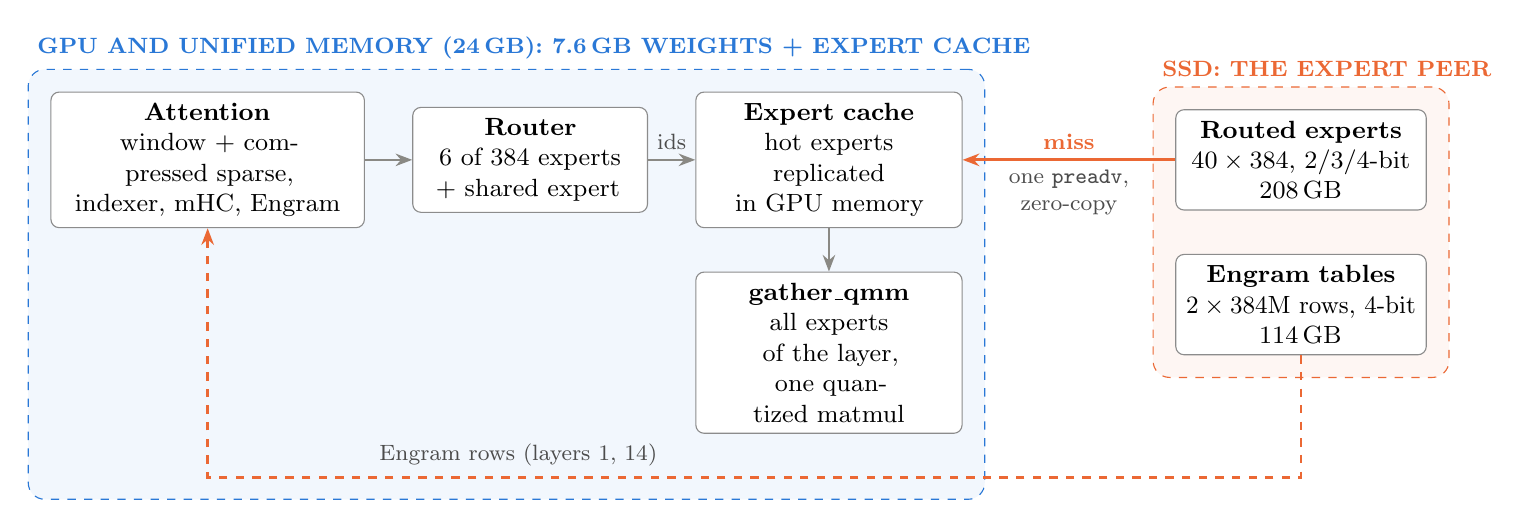
\begin{tikzpicture}[
  font=\small,
  blk/.style={draw=black!45, rounded corners=3pt, fill=white, align=center, minimum height=1.25cm, inner sep=4pt},
  arr/.style={-{Stealth[length=6pt]}, draw=dsgray, line width=0.8pt},
  rd/.style={-{Stealth[length=6pt]}, draw=dsorange, line width=1pt},
  region/.style={draw, dashed, rounded corners=6pt, inner sep=8pt}]
  \node[blk, text width=3.7cm] (att) {\textbf{Attention}\\window + compressed sparse,\\indexer, mHC, Engram};
  \node[blk, text width=2.7cm, right=0.6cm of att] (rt) {\textbf{Router}\\6 of 384 experts\\+ shared expert};
  \node[blk, text width=3.1cm, right=0.6cm of rt] (cache) {\textbf{Expert cache}\\hot experts replicated\\in GPU memory};
  \node[blk, text width=3.1cm, below=0.55cm of cache] (gq) {\textbf{gather\_qmm}\\all experts of the layer,\\one quantized matmul};
  \node[blk, text width=2.9cm, right=2.7cm of cache] (exp) {\textbf{Routed experts}\\$40\times384$, 2/3/4-bit\\208\,GB};
  \node[blk, text width=2.9cm, below=0.55cm of exp] (eg) {\textbf{Engram tables}\\$2\times384$M rows, 4-bit\\114\,GB};
  \coordinate (low) at ($(gq.south)+(0,-0.55)$);
  \draw[arr] (att) -- (rt);
  \draw[arr] (rt) -- node[above, font=\footnotesize, text=black!70] {ids} (cache);
  \draw[arr] (cache) -- (gq);
  \draw[rd] (exp) -- node[above, text=dsorange, font=\footnotesize\bfseries] {miss} node[below, align=center, font=\footnotesize, text=black!70] {one \texttt{preadv},\\zero-copy} (cache);
  \draw[rd, dashed] (eg.south) |- (low) -| node[pos=0.25, above, font=\footnotesize, text=black!70] {Engram rows (layers 1, 14)} (att.south);
  \begin{scope}[on background layer]
    \node[region, draw=dsblue, fill=dsblue!6, fit=(att)(rt)(cache)(gq)(low), label={[anchor=south west, text=dsblue, font=\footnotesize\bfseries]north west:GPU AND UNIFIED MEMORY (24\,GB): 7.6\,GB WEIGHTS + EXPERT CACHE}] {};
    \node[region, draw=dsorange, fill=dsorange!6, fit=(exp)(eg), label={[anchor=south west, text=dsorange, font=\footnotesize\bfseries]north west:SSD: THE EXPERT PEER}] {};
  \end{scope}
\end{tikzpicture}}
\caption{Overview of \method{}. Dense weights and recently used experts are kept in unified memory. After routing, missing experts are read from the SSD directly into slots of preallocated GPU buffers. Within a layer, attention, router, reads and expert computation run one after another.}
\label{fig:overview}
\end{figure}

\section{Background and motivation}
\label{sec:background}
\subsection{DeepSeek-V4.1-Flash}
DeepSeek-V4.1-Flash has 754B parameters in 40 transformer layers with hidden size 5120 \citep{deepseek41flash}. Each layer has an MoE block with one shared expert and 384 routed experts (intermediate size 2304); a sqrt-softplus router picks 6 of them for every token. Attention uses a 128-token sliding window plus \emph{compressed sparse attention}. Layers 2--19 compress the keys at ratio 2 and layers 20--39 at ratio 1. A small multihead indexer \citep{deepseek32} with 32 heads of dimension 128 then selects 512 compressed positions for each query. Selection has two levels: layer 20 picks 2048 candidate blocks of 8 positions, and later index layers only score inside those blocks. Layers 0 and 1 use the window only. Four layers (2, 8, 14 and 20) own the compressed KV caches and indexer keys, and the other layers reuse them. Layers 1 and 14 also contain an \emph{Engram} module, which looks up embeddings of hashed $n$-grams ($n\le4$) in two tables with about 384M rows each. The residual stream uses Hyper-Connections with four streams and Sinkhorn-normalized mixing matrices \citep{hyperconnections}. The model also has three DSpark draft layers for speculative decoding and a 32-layer vision encoder.

The release stores dense weights in FP8 (E4M3 with $32\times32$ E8M0 block scales) and experts in FP4 (E2M1 with one E8M0 scale per 32 values), 510\,GB in total. The reference inference code also rounds activations at fixed points during inference: FP8 before dense projections, FP4 for indexer queries and keys and for the compressed KV cache, and BF16 after each step of the indexer score. These roundings matter most where the model makes discrete choices. A score that rounds differently can change which keys the indexer selects or which experts the router picks.

\subsection{Expert parallelism in the data center}
DeepInfer \citep{deepinfer}, DeepSeek's inference engine, serves this model on a GPU cluster. Attention runs with data and context parallelism, and the MoE blocks run with expert parallelism (EP). Under EP each GPU stores a subset of the experts. After routing, an all-to-all \emph{dispatch} sends every token's hidden state to the GPUs that hold its experts, and a \emph{combine} step sends the weighted outputs back. DeepSeek uses two more techniques to keep the GPUs busy \citep{deepseekv3}. First, the computation of one micro-batch overlaps with the communication of another, so the all-to-all is hidden. Second, frequently used experts are replicated on several GPUs so that no single GPU becomes a bottleneck. Both techniques need many tokens in flight at the same time.

\subsection{Why a laptop might be enough}
Our target is a MacBook Air with an M4 chip and 24\,GB of unified memory, shared by the CPU and the GPU (about 120\,GB/s). After conversion (Section~\ref{sec:impl}) the model takes 338\,GB, far more than the memory. However, a single token needs much less than that:
\begin{itemize}
  \item The dense part (attention, shared experts, routers, mixers and Engram projections) takes 7.6\,GB at 8 bits per weight.
  \item The routed experts that one token uses take about 3.3\,GB: 40 layers times 6 experts, at 12--19\,MB per expert after compression to 2--4 bits.
\end{itemize}
The internal SSD reads 2.6--3.0\,GB/s. If the dense part stays in memory and about half of the needed experts are already cached, each token needs roughly 1.8\,GB from the SSD. That is about 0.6\,s of reading, so about one token per second looks possible.

This view treats the SSD as the device that holds the experts, the role that other GPUs play under EP. It raises the question this paper studies: \emph{which parts of expert parallelism still help when there is one GPU, one SSD and one sequence?}

\section{Design}
\label{sec:design}
Figure~\ref{fig:overview} shows the design. Dense weights stay in memory. Experts stay on the SSD, and the engine reads the ones it needs into GPU buffers. Table~\ref{tab:mapping} lists how each part of expert parallelism maps to our setting. We describe the expert path (\S\ref{sec:fetch}) and its critical path (\S\ref{sec:chain}), then the two mechanisms that shorten it: idle-window speculation, which is new (\S\ref{sec:spec}), and an expert cache that plays the role of expert replication (\S\ref{sec:replication}).

\begin{table}[t]
\centering
\small
\caption{Expert parallelism (EP) on a GPU cluster and the corresponding mechanism in \method{}.}
\label{tab:mapping}
\begin{tabular}{@{}p{0.25\linewidth}p{0.31\linewidth}p{0.37\linewidth}@{}}
\toprule
& EP on a cluster & \method{} \\
\midrule
Where experts are stored & GPU memory of many devices & SSD records (208\,GB) \\
After routing & dispatch tokens (all-to-all) & read missing experts (\texttt{preadv}, no copy) \\
Expert computation & grouped GEMM on each GPU & one \texttt{gather\_qmm} over buffer slots \\
Hiding transfers & overlap two micro-batches & compute cached experts during reads \\
Load balancing & replicate hot experts & LRU expert cache in unified memory \\
\bottomrule
\end{tabular}
\end{table}

\subsection{Reading experts instead of sending tokens}
\label{sec:fetch}
Under EP, tokens travel to the experts. On a laptop the token is already next to the GPU, so we move the expert instead.

\paragraph{Records and slabs.} We store each expert as one record on the SSD, aligned to 16\,KiB. A record holds the packed weights, scales and biases of the expert's three projections, in the same layout that MLX \citep{mlx} uses for quantized tensors. For each precision layout, the engine allocates a \emph{slab} at start-up: three GPU arrays of shape $[S,\cdot,\cdot]$, where slot $s$ holds one expert. On a cache miss, the engine takes a free slot and issues a single \texttt{preadv} call whose buffers point into the three arrays at that slot. Because the CPU and GPU share memory, the GPU reads the data exactly where the SSD wrote it, with no extra copy. We open the files with \texttt{F\_NOCACHE} so that macOS does not keep another copy in its page cache.

\paragraph{One matmul per projection.} When the router of a layer finishes, the host reads the selected expert ids. This is the only CPU--GPU synchronization in a layer. The engine maps each expert to its slot and pins the slot until the layer is done. All (token, expert) pairs of the layer then run through one \texttt{gather\_qmm} call per projection, indexed by slot, with SwiGLU and the routing weights fused into the same compiled function. This step plays the role of the combine step, without any communication.

\subsection{The critical path of one token}
\label{sec:chain}
A cluster serves many sequences, so while one micro-batch waits for the network another one computes. A laptop usually decodes one sequence, one token at a time. Figure~\ref{fig:timeline} shows what happens in four consecutive layers. The GPU first runs attention, the mixers and the router. Only then does the host know which experts are needed, and the missing ones go to the SSD. Eight I/O threads issue the reads, which finish after 10--30\,ms. The GPU then computes the experts, and the next layer can start only after that. As a result, the GPU and the SSD are rarely busy at the same time.

\begin{figure}[t]
\centering
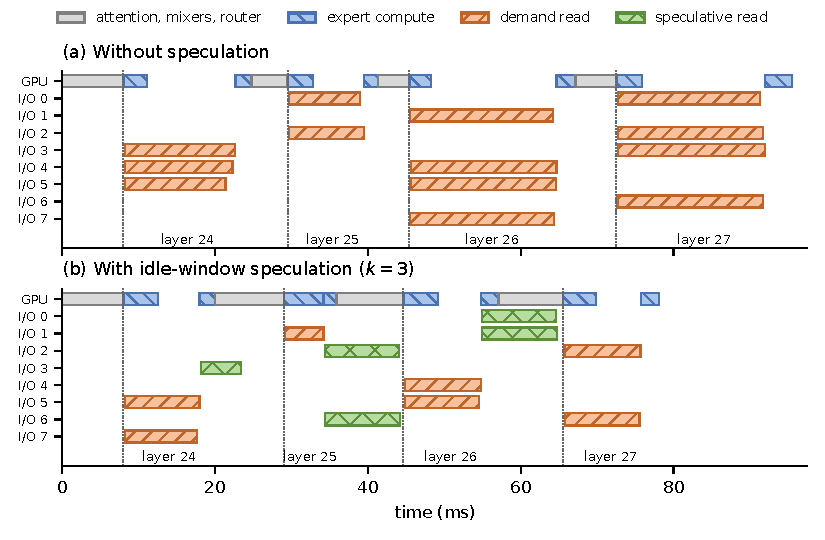
\includegraphics[width=\linewidth]{figures/timeline.pdf}
\caption{Measured timeline of four decode layers with a 5\,GB expert cache. Gray: attention, mixers and router. Blue: expert computation (cached experts first, then the missing ones). Orange: demand reads, one row per I/O thread. Green: speculative reads (\S\ref{sec:spec}). (a) Reads start only after the router of their layer finishes, and the SSD is idle while the GPU works. (b) With idle-window speculation, guesses for the next layer fill this idle time; several experts of each layer are already in memory when the router finishes. Each panel shows the median of three traced tokens. To time GPU work we synchronize after each expert group, which makes a step 2\% (a) and 14\% (b) slower than untraced decoding in the same run.}
\label{fig:timeline}
\end{figure}

This dependency gives a simple cost model. Let $a$ be the time of attention, mixers and router in one layer, $c$ the expert computation time, $m_\ell$ the number of missing experts in layer $\ell$, $b$ the size of one expert and $B$ the SSD bandwidth. A decode step then takes about
\begin{equation}
t_{\text{token}} \;\approx\; \sum_{\ell=1}^{40}\Big(a + c + \frac{m_\ell\, b}{B}\Big).
\label{eq:chain}
\end{equation}
On an idle machine we measured 0.80\,s per token. The compute terms add up to 0.25\,s. With a 49\% hit rate the missing experts total 1.78\,GB; the measured SSD wait was 0.55\,s, which corresponds to 3.2\,GB/s. These numbers roughly add up to the measured step, and they show three ways to make it shorter. The first is fewer misses, which needs a larger cache (\S\ref{sec:replication}). The second is to overlap the reads of a layer with the computation that does not depend on them; inside one layer, that is only the cached experts. The third is to read experts \emph{before} the router asks for them, so that the SSD also works while the GPU computes (\S\ref{sec:spec}).

Section~\ref{sec:parallel-eval} measures each of these options, together with other kinds of parallelism from related systems.

\subsection{Idle-window speculation}
\label{sec:spec}
Equation~\eqref{eq:chain} also shows when the SSD is idle: during $a$ and $c$, while the GPU runs attention and computes experts. In a decode step this idle time adds up to about 0.25\,s, enough to read about 50 experts. Reading the next layer's experts during this time would take reads off the critical path. Prefetching experts is not new \citep{moeoffload,pregated,moeinfinity,promoe,adapmoe}. In particular, \citet{moeoffload} already guess the next layer's experts by applying its gate to the current hidden state, and we use the same predictor. However, prefetching the most likely next-layer experts made decode 5--6\% \emph{slower} in our measurements. Looking at the trace, we suspected two causes, which the ablation in Section~\ref{sec:parallel-eval} later separated:
\begin{itemize}
  \item \textbf{Guesses ran before needed reads.} The engine issued the guesses for layer $\ell+1$ before the misses of layer $\ell$. Both went to the same I/O queue, so every wrong guess delayed a read the token was waiting for.
  \item \textbf{Guesses might pollute the cache.} A guessed expert entered the LRU list as most recently used, so a wrong guess could push out an expert that had been used. The ablation shows that this effect is small at a 5\,GB cache.
\end{itemize}
\emph{Idle-window speculation} addresses both and needs no training or model change. Its essential part is the first: issue guesses only after the demand reads have landed. After the router of layer $\ell$ finishes, the engine also applies the router of layer $\ell+1$ to the current hidden state, using its exact scoring (sqrt-softplus plus bias), and takes the top $k$ experts as guesses. The guesses go to a separate thread that waits until all misses of layer $\ell$ have arrived and only then issues their reads. They therefore run while the GPU computes, in the window where the SSD would otherwise be idle. In addition, a guessed expert is inserted at the \emph{cold} end of the LRU list, the end that is evicted first, similar to low-priority insertion in CPU caches \citep{qureshi2007}. If layer $\ell+1$ uses it, it moves to the hot end; if not, the next guess or miss replaces it before any used expert. A guess never evicts a slot that is pinned or in use by the current request. The change is about 40 lines in the expert store and the MoE block. The ablation in Section~\ref{sec:parallel-eval} shows that the first fix, waiting for the demand reads, provides most of the gain; cold insertion adds a little on top and hurts on its own. Figure~\ref{fig:timeline}b shows the effect: in the same four layers, guessed experts arrive during the GPU's work, and the demand reads that remain are fewer and shorter.

\subsection{Replication: spending memory on the cache}
\label{sec:replication}
Replicating hot experts is the part of EP that transfers most directly. A cluster copies busy experts so that no GPU waits; we keep recently used experts in memory so that no read is needed. Each hit removes one term $b/B$, about 5\,ms, from Equation~\eqref{eq:chain}. We use least-recently-used replacement. On routing traces recorded from the real model, LRU had a higher hit rate than least-frequently-used at the same capacity, and capacity mattered more than the policy: 1.5 times more slots raised the hit rate from 0.38 to 0.47.

Because cache size drives decode speed, the rest of the design tries to save memory:
\begin{itemize}
  \item Dense FP8 weights convert to MXFP8 without loss (Section~\ref{sec:impl}), so we never keep a higher-precision copy.
  \item Expert reads skip the page cache, so the same expert is never stored twice.
  \item Speculative reads enter the cache cold (\S\ref{sec:spec}), and speculative decoding is off by default, so neither pushes useful experts out.
\end{itemize}
The cache size is set at start-up from the memory that is free at that moment, minus a 4\,GB margin, and at least 9\,GB always stay free for macOS. With less than that the system starts swapping and decode slows down sharply. On an idle 24\,GB machine this gives 5--6\,GB of expert slots.

We also provide an optional approximation based on the same idea. If a missing expert carries less than 8\% of a token's routing weight, the engine skips it and saves the read. It lowers top-1 agreement with the API on open-ended text by 2.4 points. We did not measure its speed effect in an interleaved test, so we report no speed-up for it, and it is off by default.

\section{Implementation}
\label{sec:impl}
\method{} is about 3,800 lines of Python on top of MLX \citep{mlx}, plus one Metal kernel that Section~\ref{sec:indexer} describes. We ported the official reference implementation operation by operation, because we wanted every later speed-up to be checkable against it. The engine is not lossless as a whole, since the experts are compressed, but everything else is meant to compute exactly what the reference computes.

\paragraph{Weight format.} Table~\ref{tab:format} shows where each part of the model ends up. The FP8 dense weights convert to MLX's MXFP8 format without any loss, because both formats store the same E4M3 values and differ only in how they share scales. The experts are requantized from FP4 to two to four bits per weight. For every group of weights the converter searches for the clipping ratio with the smallest reconstruction error, and it chooses the bit width of each layer by comparing hidden states against the original experts, as the appendix describes. Lossless MXFP4 experts would not have fit on our disk next to the download stream, but they are a one-line change for machines with more storage. The Engram tables are stored as 4-bit rows and stay within a fraction of a percent of the originals.

\begin{table}[t]
\centering
\small
\caption{Converted weights of DeepSeek-V4.1-Flash as stored on disk. Sizes are in GiB, which we write as GB throughout.}
\label{tab:format}
\begin{tabular}{@{}p{0.43\linewidth}lrl@{}}
\toprule
Component & Format & Size & Location \\
\midrule
Dense layers: attention, shared experts, routers, mHC, Engram projections & \texttt{mxfp8}, lossless & 6.9 & memory \\
Output head and other global tensors & affine 8-bit / BF16 & 0.7 & memory \\
Embedding & BF16, memory-mapped & 1.2 & SSD \\
Routed experts, $40\times384$ & affine 2/3/4-bit, $g=64$ & 208.3 & SSD \\
DSpark layers: dense parts / experts ($3\times128$) & \texttt{mxfp8} / affine 2/3-bit & 0.7 / 4.5 & SSD \\
Vision encoder & BF16 & 0.9 & SSD \\
Engram tables, $2\times384$M rows & affine 4-bit, $g=32$ & 114.4 & SSD \\
\midrule
Total on disk & & 337.6 & \\
\bottomrule
\end{tabular}
\end{table}

\paragraph{One forward path.} As in DeepInfer, prefill, decode, chunked prefill, prefix reuse and speculative verification all share one forward function that can process any chunk of tokens at any position. The state of a sequence, which includes the sliding-window buffers, the compressed caches and the compressor's unfinished tail, can be saved and restored exactly. Two features build on this. With \emph{bounded replay}, the later half of the layers processes only the last 140 tokens of a prompt, because those layers see older tokens only through compressed caches that earlier layers have already filled. This roughly halves the expert reads of a long prefill. With \emph{conversation reuse}, the engine keeps the last sequence and a snapshot taken just before the end of the last prompt, so a follow-up turn only processes its new tokens. The snapshot matters in thinking mode, where the chat template removes the previous turn's reasoning from the next prompt.

\paragraph{Other components.} Engram rows are read from the SSD through a row cache. DSpark drafts are verified with speculative rejection sampling, which keeps the output distribution exact, and a small controller turns speculation off when it is slower than plain decoding. The server speaks the OpenAI, Anthropic and Responses APIs and reuses DeepSeek's own prompt rendering and output parsing \citep{deepseekrecipe}, while structured outputs use XGrammar \citep{xgrammar}. The converter never stores the 510\,GB release: it reads each tensor from the model hub with range requests, converts it on the GPU, writes it to its final place, and can resume after any interruption.

\paragraph{Testing.} The test suite runs DeepSeek's PyTorch model, with CPU versions of its GPU kernels, on small random configurations that exercise every mechanism of the model. With activation rounding switched off on both sides, prefill and decode logits agree with a median cosine above 0.9999, the vision encoder matches exactly, and greedy speculative decoding produces the same tokens as greedy decoding. On the real checkpoint, every converted layer agrees with the reference on a real chat prompt, and the Engram hash ids are identical.

\section{Case study: the sparse-attention indexer}
\label{sec:indexer}
Long prompts take minutes on a laptop, and part of that time goes to the indexer. For a query with indexer heads $\q_1,\dots,\q_H\in\RR^{d}$ and signed head weights $w_1,\dots,w_H$, the reference scores each visible compressed key $\kv_j$ as
\begin{equation}
s_j \;=\; \bfround\!\Big(\sum_{h=1}^{H} \bfround\big(\relu{\bfround(\q_h^\top\kv_j)}\, w_h\big)\Big),
\label{eq:score}
\end{equation}
with the outer sum accumulated in FP32, and keeps the best $K$ keys. Prefill scores every query against every visible key, so this cost grows with the square of the prompt length. We tried two ways to make it cheaper. The first computes Equation~\eqref{eq:score} faster without changing any result, and the second skips keys that cannot make the cut.

\subsection{Faster scoring with the same results}
\paragraph{BF16 products.} The reference computes each product $\q_h^\top\kv_j$ in FP32 and then rounds it to BF16. Both inputs are FP4 values with power-of-two scales, which BF16 represents exactly, and the following lemma shows when a BF16 matrix multiplication returns the same rounded result.
\begin{lemma}
\label{lem:exact}
Let $\q,\kv\in\RR^{128}$ hold E2M1 values with one power-of-two scale per block of 32 elements, and let $\sigma_b$ be the product of the two scales of block $b$. Assume that $\max_b\sigma_b/\min_b\sigma_b\le 2^{9}$ and that every block product stays in the normal FP32 range. Then every partial sum of $\q^\top\kv$, in any order, is exactly representable in FP32, and a BF16 matrix multiplication that accumulates in FP32 and rounds once returns $\bfround(\q^\top\kv)$, the reference result.
\end{lemma}
The appendix gives the proof. MLX's BF16 matrix kernels accumulate in FP32, although we checked this empirically rather than for every kernel variant. Where the scale condition fails, both computations are ordinary FP32 sums whose last bit can depend on the order of summation, just as it can between different GPU kernels running the reference. On indexer inputs captured from a real 32K-token prompt, the BF16 version reproduced every one of about a billion scores.

\paragraph{Fused head reduction.} After the matrix multiplication, Equation~\eqref{eq:score} still needs a ReLU, a weighting and a rounding for every element, followed by a sum over heads. Written as array operations, this reads a large intermediate tensor three times. We replaced it with a single Metal kernel in which each thread handles one pair of query and key and walks over the heads, applying the same roundings in the same order. On every input we tested it matches the array version. Both sum the heads in FP32, so their results could differ in the last bit only if the summation orders differed and the terms spanned a very wide range, which is equally true of the reference. Figure~\ref{fig:indexer}a shows that together the two changes make an indexer block about twice as fast on real inputs, with the same selected keys.

\paragraph{Fixed tie order.} A partition-based Top-$K$ leaves ties at the boundary to the kernel. We sort by a 64-bit key built from the BF16 score and the position, so that ties go to the earlier position and a NaN score is never selected. Selection thereby becomes a pure function of the scores, which an exact screening method must also reproduce.

\subsection{Skipping keys: exact screening}
\label{sec:dosa}
DoSA \citep{dosa} skips keys while keeping the selection exact. A seed set of keys gives a lower bound $\tau$ on the $K$-th best score, a cheap upper bound $U_j$ is computed for every other key, and keys with $U_j<\tau$ are dropped before full scoring. DoSA reports large speed-ups on GLM-5.2 and DeepSeek-V3.2 at contexts of half a million tokens and more. V4.1-Flash differs in three ways that could matter: it has fewer indexer heads, a smaller $K$, and its own two-level candidate selection. We therefore measured how well such a bound works on this model.

\paragraph{Setup.} We captured the indexer inputs of a real 32K-token prompt and studied every index layer except the one that chooses the candidate blocks, which needs all block maxima and cannot skip keys. For each layer we used the last decode query and sixteen queries from the prompt. A key is \emph{eligible} for a query if the query can see it and, in the later layers, if it lies inside the query's candidate blocks. As in DoSA, the bound evaluates the positive heads $P$ and the strongest negative heads $E$ exactly, and merges the remaining negative heads into a single term:
\begin{equation}
U_j = \sum_{h\in P} w_h\relu{\q_h^\top\kv_j} - \sum_{h\in E} |w_h|\relu{\q_h^\top\kv_j} - \relu{\textstyle\sum_{h\in N\setminus E}|w_h|\,\q_h^\top\kv_j}.
\end{equation}
The bound is valid because $\sum_i \relu{x_i}\ge\relu{\sum_i x_i}$. We enlarged it slightly to cover the BF16 roundings of Equation~\eqref{eq:score} and checked that no dropped key belongs to the true Top-$K$. Its cost counts the fully scored seed keys, the dot products of the bound for every other eligible key, and the remaining heads for every key that survives.

\paragraph{Results.} Figure~\ref{fig:indexer}b and the appendix show the cost at the best head budget for each layer. A useful bound needs about two thirds of the heads, and even then screening saves only a tenth to a fifth of the indexer's work, before the overhead of compacting the survivors on the GPU. DoSA's joint bound for omitted positive heads did not drop a single additional key on this model, and a low-rank bound built from the leading singular vectors of the query heads failed as well, because those singular values decay slowly. Two properties of the model explain the difference from DoSA's setting. At these context lengths, $K$ is a large fraction of the keys, so the threshold $\tau$ sits low in the score distribution. And the model's own candidate selection already removes many keys before the indexer score matters. Since the indexer is only a small part of a 32K-token prefill, the end-to-end gain would be around one percent. We left screening off and shared the measurements with the DoSA authors. The picture may change at contexts of 128K tokens and more, but prefilling such a prompt takes hours on this machine.

\begin{figure}[t]
\centering
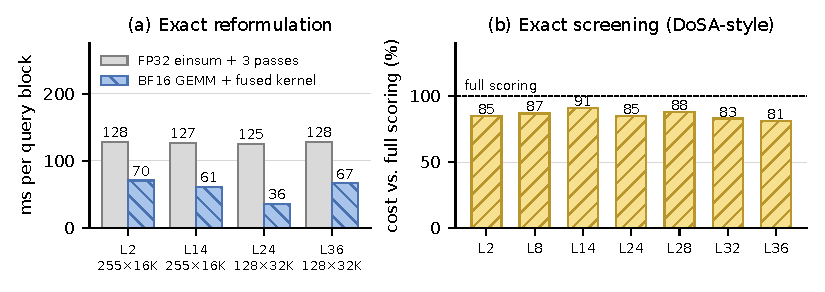
\includegraphics[width=\linewidth]{figures/indexer.pdf}
\caption{(a) Indexer time per prefill query block on real inputs, before and after the BF16 matmul and the fused head reduction. Labels give the layer and the block shape as rows times keys. Scores and selected keys are identical on these blocks. The matmul alone runs 1.5 to 1.9 times faster and the head reduction 5 to 6 times faster. (b) Cost of an exact screening bound relative to fully scoring the eligible keys, per index layer, at the best head budget. The bound was checked offline in float64 with slack for the BF16 roundings; the cost includes scoring the seed keys and is averaged over 17 queries of a 32K-token prompt with $K=512$.}
\label{fig:indexer}
\end{figure}

\section{Evaluation}
\label{sec:eval}
\paragraph{Setup.} All experiments run on the MacBook Air of Table~\ref{tab:model} with other applications closed. For the main decode experiments, all compared settings run interleaved in one process, so that they see the same cache state and the same background load. Each block decodes six tokens with one setting, the order of settings rotates every round, and we use three prompts in English and Chinese. We report the mean over blocks of the median time per token, with 95\% confidence intervals from Student's $t$ distribution, and we compare every block with the block of the reference setting from the same round. The evaluation answers three questions: how fast the system is, which kinds of parallelism help, and how close its output is to DeepSeek's own deployment.

\subsection{Speed and the cost model}
\label{sec:e2e}
Table~\ref{tab:results} summarizes the end-to-end results. With an expert cache that still leaves 9\,GB to macOS, \method{} decodes 1.23 tokens per second. Figure~\ref{fig:sweep} shows how decode speed depends on the size of the cache. Speed rises steadily as the cache grows, because every additional hit removes a read from the chain. Idle-window speculation shifts the whole curve upward. It is faster at every cache size, in 43 of 45 paired blocks, and it cuts the time spent waiting for the SSD by roughly a quarter.

\begin{table}[t]
\centering
\small
\caption{End-to-end results on a MacBook Air with 24\,GB. Decode uses idle-window speculation unless noted. Quality numbers come from teacher forcing against continuations sampled from DeepSeek's API.}
\label{tab:results}
\begin{tabular}{@{}lr@{}}
\toprule
Decode, 5.5\,GB expert cache, 9\,GB left to macOS & 1.23 tokens/s \\
Decode, 5.5\,GB expert cache, without speculation & 1.08 tokens/s \\
Decode, 6.5\,GB expert cache & 1.35 tokens/s \\
Speed-up from speculation, 2.5 to 6.5\,GB caches & 11--27\% \\
First token for a 14-token, 1K-token and 16K-token prompt & 10\,s, 49\,s, 9\,min \\
SSD read bandwidth with one or several reads in flight & 2.7, 3.0\,GB/s \\
Top-1 agreement on 129 open-ended continuation tokens & 86.0\% \\
Mean top-1 agreement over all 17 cases & 96.7\% \\
Mean NLL per token, ours and DeepSeek's API & 0.127, 0.046 \\
Needle retrieval, 12 lengths up to 16,385 tokens & 12 of 12 correct \\
\bottomrule
\end{tabular}
\end{table}

The cost model of Equation~\eqref{eq:chain} describes the runs without speculation closely. A two-parameter fit to the bytes each token has to read matches all five cache sizes within two percent. Applied to the runs with speculation, the same fit predicts that they should be even faster than they are, because it ignores the speculative reads. Those reads are not free: about half of their volume still costs time, and the other half falls into time when the SSD would have been idle. The traces confirm this directly. Without speculation the SSD is busy for less than two thirds of a decode step, and with speculation the busy share rises by roughly a fifth, almost all of it taken up by reads that overlap no demand read.

\begin{figure}[t]
\centering
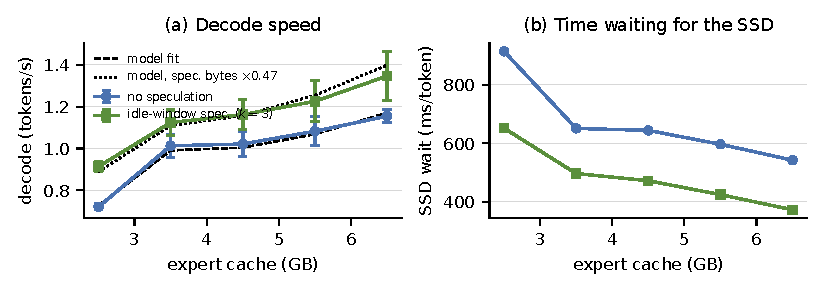
\includegraphics[width=0.9\linewidth]{figures/sweep.pdf}
\caption{(a) Decode speed against expert cache size, with and without idle-window speculation, interleaved in one process with 95\% confidence intervals over nine blocks. The dashed line is the cost model $t=C+D/B$ fitted to the runs without speculation, with $C=117$\,ms and $B=2.37$\,GB/s, which matches them within 2\%. The dotted line adds the speculative bytes with weight $\alpha=0.47$, fitted on the same runs. (b) Time per token spent waiting for the SSD.}
\label{fig:sweep}
\end{figure}

\paragraph{Prefill.} Prefill behaves differently from decode. Even a short prompt routes to most experts of every layer, so the first chunk reads nearly the whole expert set once, and long prompts are limited by GPU compute rather than by the SSD. Bounded replay keeps the later layers out of most of that work. We prefill in chunks of 4K tokens, because a single long chunk is no faster and needs considerably more memory at its peak.

\subsection{Where does parallelism help?}
\label{sec:parallel-eval}
We now return to the question of the introduction and look at each level of the system where parallelism could help. Table~\ref{tab:ablation} and Figure~\ref{fig:parallel} show the interleaved ablation of the decode schedule, and Table~\ref{tab:negative} collects the other techniques we tried.

\begin{table}[t]
\centering
\small
\caption{Decode schedules at a 5\,GB cache, interleaved in one process. Speed-ups are paired against the serial schedule of the same round, with 95\% confidence intervals over 12 blocks. All speculative schedules read three guesses per layer. In the first run the naive prefetcher ranks its guesses by the raw gate logits; the second run repeats the key schedules with the router's exact scoring for every prefetcher. Tokens per second and SSD wait are from the first run.}
\label{tab:ablation}
\resizebox{\linewidth}{!}{%
\begin{tabular}{@{}lccrrrr@{}}
\toprule
Schedule & Guesses wait & Guesses cold & Tokens/s & SSD wait, ms & Speed-up, run 1 & Speed-up, run 2 \\
\midrule
Serial & & & 1.03 & 630 & 1.00 & 1.00 \\
Overlap cached and missing experts & & & 1.07 & 617 & $1.05\pm0.04$ & \\
Naive next-layer prefetch \citep{moeoffload} & no & no & 0.97 & 667 & $0.95\pm0.07$ & $0.89\pm0.05$ \\
Guesses issued with the demand reads & no & no & 0.99 & 637 & $0.96\pm0.05$ & \\
Guesses inserted cold only & no & yes & 0.87 & 770 & $0.85\pm0.06$ & \\
Guesses wait for demand reads only & yes & no & 1.17 & 464 & $1.15\pm0.05$ & $1.10\pm0.05$ \\
\textbf{Idle-window speculation} & yes & yes & \textbf{1.20} & \textbf{456} & $\mathbf{1.17\pm0.05}$ & $\mathbf{1.14\pm0.05}$ \\
\bottomrule
\end{tabular}}
\end{table}

\begin{figure}[t]
\centering
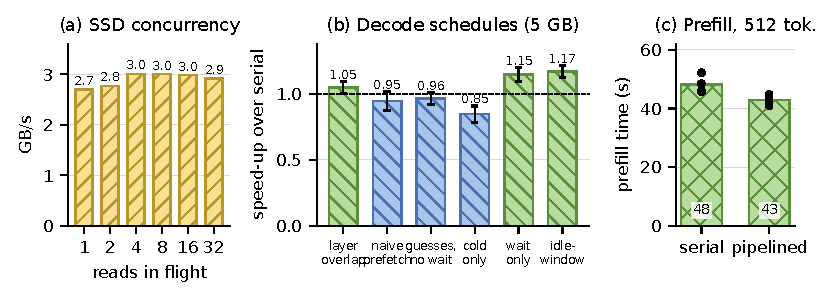
\includegraphics[width=\linewidth]{figures/parallel.pdf}
\caption{Parallelism on one laptop. (a) Read bandwidth for expert records against the number of reads in flight. (b) The first run of the schedule ablation in Table~\ref{tab:ablation}, as speed-up over the serial schedule with 95\% confidence intervals; green marks schedules that are faster than serial. (c) Prefill of a 512-token prompt with and without reading the next batch of experts while the current one computes; bars show means and dots individual runs.}
\label{fig:parallel}
\end{figure}

\paragraph{Inside the SSD.} The drive itself is the one place where parallelism comes for free. It delivers expert records noticeably faster with several requests in flight than with one, and it saturates after a few, which our eight I/O threads easily provide. Splitting a single expert into smaller reads adds nothing, because a read of an entire expert is already large.

\paragraph{Inside a layer.} Computing the cached experts while the missing ones load is the closest match to the cluster's micro-batch overlap. It helps a little. Figure~\ref{fig:timeline}a shows why it cannot help more: the cached experts of a layer take a few milliseconds to compute, while the reads take several times longer.

\paragraph{Across layers.} This is where the schedule matters most. Naive prefetching of the next layer's experts is slower than not prefetching at all, in both runs of the ablation. It even collects twice as many speculative hits as idle-window speculation and still loses, because its guesses compete with the reads the token is waiting for. Making the guesses wait for those reads is what turns the loss into a gain, and it accounts for almost all of the improvement. Inserting the guesses cold adds a little on top, within the confidence interval. On its own, cold insertion is harmful, because guesses that arrive too early are evicted again before the next layer can use them. With both changes, idle-window speculation was faster than the serial schedule in 23 of 24 paired blocks across the two runs, and it produced exactly the same tokens as decoding without it. Three guesses per layer worked best; with more, the guesses again started to delay demand reads.

\paragraph{Across expert batches in prefill.} During prefill a whole chunk of tokens goes through each layer, which gives the engine something like a batch. Reading the next batch of experts while the current one computes made prefill about a tenth faster on an otherwise idle machine. In an earlier session with other programs holding memory, the same pipelining caused swapping and gained nothing, because the extra batch needs room.

\paragraph{Across tokens.} Speculative decoding checks several drafted tokens in one pass \citep{specdecoding}. On a GPU this amortizes weight reads over several tokens. Here the drafted tokens route to different experts, so the check must read the union of their experts, and decode became several times slower. The controller described in Section~\ref{sec:impl} detects this and falls back to plain decoding.

\paragraph{In the operating system.} The page cache could in principle serve as a larger second-level cache behind the slab. In practice it competes with the slab for the same memory, and no setting we tried was faster than bypassing it.

\begin{table}[t]
\centering
\small
\caption{Other techniques, each measured against a baseline from the same session in tokens per second, or in seconds for prefill.}
\label{tab:negative}
\resizebox{\linewidth}{!}{%
\begin{tabular}{@{}p{0.42\linewidth}rrp{0.28\linewidth}@{}}
\toprule
Technique & Without & With & Note \\
\midrule
Pipelined expert batches in prefill, 512 tokens & 48.1\,s & 42.8\,s & interleaved, four runs each \\
Four-way split reads per expert & 1.12 & 1.11 & \\
OS page cache behind a 5\,GB slab & 1.12 & 0.20--0.61 & \\
DSpark speculative decoding, fixed draft length & 1.28 & 0.35 & \\
Two, three, four or six guesses per layer & & 1.13, 1.19, 1.14, 1.06 & same day, not interleaved \\
\bottomrule
\end{tabular}}
\end{table}

Taken together, the measurements give a simple rule. Parallelism pays off when it gives the SSD work during time that the dependency chain would leave idle, without delaying a read the token is waiting for and without taking memory from the cache. Idle-window speculation meets all three conditions, while naive prefetching, speculative decoding and the page cache each break one of them. Even so, the size of the cache remains the strongest single factor.

\subsection{Output quality}
\label{sec:quality}
We compare \method{} with DeepSeek's own deployment using continuations sampled from DeepSeek's API, published with the ds4 project \citep{ds4}, and run them through the converted model with teacher forcing. Figure~\ref{fig:api} shows top-1 agreement for each case. On the five open-ended continuations, our model picks the same next token as the API for 86\% of the tokens. The gap comes from compressing the experts to two or three bits, which matters more for free text than for retrieval. The other twelve cases are needle-retrieval prompts whose lengths sit just around the sliding window, the boundaries of the key selection and the candidate-block level. The model answers all of them correctly, which shows that the long-context machinery works as in the reference.

\begin{figure}[t]
\centering
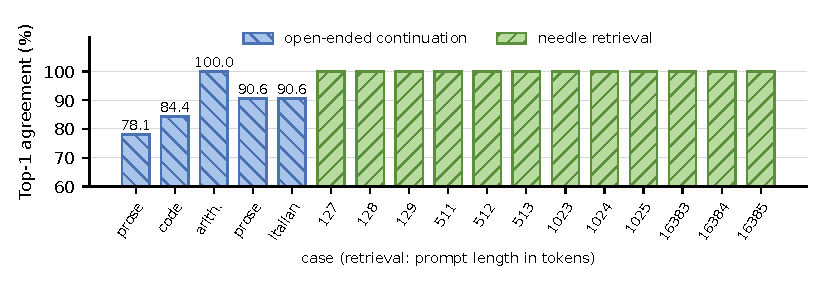
\includegraphics[width=0.9\linewidth]{figures/api_cases.pdf}
\caption{Top-1 agreement with continuations sampled from the official API. The retrieval prompts have one-token answers.}
\label{fig:api}
\end{figure}

\section{Related work}
\label{sec:related}
\paragraph{Running models larger than memory.} FlexGen offloads weights, activations and the KV cache to CPU memory and disk and searches for a schedule that maximizes throughput for large batches \citep{flexgen}. LLM in a Flash keeps weights in flash storage and loads only the rows that predicted-active neurons need, reading them in large chunks \citep{llmflash}. PowerInfer keeps frequently activated neurons on the GPU and computes the rest on the CPU \citep{powerinfer}. For MoE models, \citet{moeoffload} combine an LRU expert cache with speculative prefetching of the next layer's experts on consumer GPUs; our predictor is theirs. Pre-gated MoE changes the model so that each layer selects the next layer's experts \citep{pregated}, MoE-Infinity and ProMoE prefetch and cache experts from activation statistics \citep{moeinfinity,promoe}, AdapMoE adapts gating and prefetching to the cache \citep{adapmoe}, Fiddler runs experts on the CPU instead of moving them \citep{fiddler}, MoE-Lightning pipelines CPU and GPU work for large batches \citep{moelightning}, and EdgeMoE and PowerInfer-2 bring expert or neuron offloading to phones \citep{edgemoe,powerinfer2}. llama.cpp memory-maps quantized weights and lets the operating system decide what stays in memory \citep{llamacpp}. Our setting differs in two ways. The dense part alone uses a third of the memory, and the workload is a single interactive sequence. Under these conditions, our measurements favour a fixed set of cache slots filled by reads that bypass the page cache over OS caching or cross-layer prefetching.

\paragraph{Expert parallelism.} DeepSeek's serving stack spreads experts over many GPUs, overlaps all-to-all communication with computation using two micro-batches, and replicates heavily used experts \citep{deepseekv3,deepinfer}. We map these ideas to one GPU and one SSD and measure which of them still apply.

\paragraph{DeepSeek-V4 models on Apple silicon.} Several community projects run DeepSeek-V4-generation models on Macs, and we learned from all of them. ds4 is a dedicated C and Metal engine whose API-sampled test vectors we use for evaluation \citep{ds4}. flash-moe streams experts from the SSD in C and Metal \citep{flashmoe}. Two MLX ports target V4-Flash and V4.1-Flash \citep{ssdmoe,pipenetwork}. \method{} follows the official reference implementation and its numerics op by op, which lets us test against it, and it shares its forward path and serving interface with DeepInfer \citep{deepinfer} and deepseek-recipe \citep{deepseekrecipe}.

\paragraph{Quantization.} Post-training methods such as GPTQ lower weight precision with second-order error correction \citep{gptq}. We use a simpler per-group clipping search because the converter streams each expert once from the network and has no calibration pass. We instead choose precision per layer and keep the dense weights lossless.

\paragraph{Sparse-attention indexers.} DeepSeek Sparse Attention selects keys with a light multihead indexer \citep{deepseek32}. V4.1-Flash adds key compression and two-level candidate selection \citep{deepseek41flash}, and IndexCache reuses indices across layers \citep{indexcache}. Several methods speed up selection while keeping the full scorer's output. GVR checks a predicted threshold during decoding \citep{gvr}, LiteTopK fuses scoring with candidate filtering \citep{litetopk}, and DoSA drops keys using score bounds \citep{dosa}, following the MaxScore and WAND idea from document retrieval \citep{maxscore1995,wand2003}. MISA screens with a subset of heads but does not guarantee the full scorer's selection \citep{misa}.

\paragraph{Prefetch control.} Giving demand requests priority over prefetches and inserting prefetched data with low priority are established techniques in processor memory systems \citep{padc,fdp,qureshi2007}. Idle-window speculation applies both to expert reads from an SSD. Our contribution there is the measurement that shows why naive expert prefetching loses on a memory-bound laptop and that these two known fixes turn the loss into a gain, not the fixes themselves.

\section{Limitations and conclusion}
\label{sec:conclusion}
\paragraph{Limitations.} \method{} decodes at roughly a token per second, which suits interactive use with short answers and offline jobs but not serving many users. It runs one sequence at a time, and long prompts take minutes. The compressed experts cost some agreement with the API on open-ended text, although retrieval is unaffected, and machines with more storage can keep the experts lossless. All results come from a single machine, with short prompts and short decode blocks, and we did not measure decode at long context. We also did not compare against other engines: the community projects we cite run related checkpoints with different quantization on other hardware, and porting them to this setting was beyond our scope. A Mac with a faster SSD or more memory would shift the balance between the techniques we measured. Finally, our screening study covers contexts up to 32K tokens and does not settle the question for much longer ones.

\paragraph{Conclusion.} We asked what expert parallelism becomes on a laptop whose only other device is an SSD. Reading experts straight into fixed GPU buffers replaces the token dispatch of a cluster, and an LRU cache replaces expert replication. A single decoding token turns each layer into a chain of computing, reading and computing again, and the SSD spends a third of every step waiting. The overlap techniques of a cluster recover little of that time, and naive prefetching even makes it worse, because its guesses delay the reads a token needs. Letting the guesses wait until those reads have landed is enough to fill the idle time, and it makes decode clearly faster without changing a single output token. With these pieces, a 24\,GB MacBook Air runs the 754B-parameter DeepSeek-V4.1-Flash at about 1.2 tokens per second, close to DeepSeek's own deployment. We release the engine, the converter, the tests and all measurement logs.

\label{lastmainpage}
\clearpage
\section*{AI use statement}
We used generative AI tools for drafting code, experiments and this manuscript, which were reviewed and revised by the author. The author takes responsibility for the final manuscript and implementation.

\section*{Reproducibility statement}
The engine, converter and tests are released under the Apache 2.0 license at \url{https://github.com/haoruilee/DeepInfer-Mac}. Section~\ref{sec:impl} and Appendix~\ref{app:format} describe the weight format, and \texttt{python -m deepinfer\_mac convert} reproduces the checkpoint from the public release. \texttt{tests/} runs the parity tests against the official reference implementation when its source is available (set \texttt{DSV41\_REF}); otherwise those tests are skipped. The measurements use these scripts; their raw outputs (logs and JSON files) are included in \texttt{paper/logs}. One interleaved ablation run (\texttt{ablation2.json}) was disturbed by an external event, with blocks below 0.1 tokens/s in every configuration; we repeated it (\texttt{ablation3.json}) and do not use it. The scripts are:
\begin{itemize}
  \item \texttt{scripts/spec\_ablation.py} and \texttt{scripts/spec\_sweep.py}: the interleaved schedule ablation (Table~\ref{tab:ablation}) and the cache-size sweep (Figure~\ref{fig:sweep}), with raw per-token times and store counters;
  \item \texttt{scripts/trace\_decode.py}: the per-layer timelines (Figure~\ref{fig:timeline});
  \item \texttt{scripts/bench\_io\_parallel.py} and \texttt{scripts/prefill\_overlap.py}: SSD concurrency and prefill pipelining (Figure~\ref{fig:parallel});
  \item \texttt{scripts/decode\_speed.py}, \texttt{scripts/spec\_ab.py}, \texttt{scripts/schedule\_ab.py}: earlier decode measurements;
  \item \texttt{scripts/trace\_policies.py}: replacement-policy replay on recorded routing traces;
  \item \texttt{scripts/score\_api.py}: agreement with the API-sampled vectors of \citet{ds4}; \texttt{scripts/real\_check.py}: per-layer parity on the real checkpoint; \texttt{scripts/quant\_damage.py}: per-layer effect of expert compression;
  \item \texttt{scripts/capture\_indexer.py} and \texttt{scripts/dosa\_study.py}: the indexer study (the captured inputs, about 300\,MB, are not included); \texttt{scripts/bench\_kernels.py}: the indexer and MXFP8 kernel timings.
\end{itemize}
\texttt{paper/figures/make\_plots.py} draws the figures; values it does not read from \texttt{paper/figures/data} are copied from the logs named above. The numbers in Section~\ref{sec:quality} come from the v0.1.1 build (\texttt{final\_eval.log}); a later build scored 97.1\% mean agreement (\texttt{after\_score.log}).

\clearpage
\bibliography{references}
\bibliographystyle{iclr2027_conference}
\clearpage
\appendix
\section{Weight layout}
\label{app:format}
Each routed expert is one record of three projections: gate $W_1$ and up $W_3$ ($2304\times5120$) and down $W_2$ ($5120\times2304$). Each projection is stored as packed integers, per-group scales and per-group biases in MLX's affine format with group size 64, and the record is padded to a multiple of 16\,KiB. Table~\ref{tab:layers} gives the bit widths per layer. We chose them with \texttt{scripts/quant\_damage.py}, which runs real layers once with the converted experts and once with the original FP4 experts and compares hidden states layer by layer. The first four layers, the layers that own KV caches or index keys, and the decoder band received 3 bits, the last layer 4 bits, and the rest 2-bit gate/up projections. The DSpark draft experts use 2-bit gate/up and 3-bit down projections.

\begin{table}[h]
\centering
\small
\caption{Expert bit widths ($W_1$/$W_3$/$W_2$) and record sizes.}
\label{tab:layers}
\begin{tabular}{@{}llr@{}}
\toprule
Layers & Bits & Record \\
\midrule
0--3, 8, 14, 20--38 & 3/3/3 & 15.5\,MB \\
4--7, 9--13, 15--19 & 2/2/3 & 12.5\,MB \\
39 & 4/4/4 & 19.9\,MB \\
\bottomrule
\end{tabular}
\end{table}

\section{Proof of Lemma~\ref{lem:exact}}
\label{app:exact}
E2M1 magnitudes are $\{0, 0.5, 1, 1.5, 2, 3, 4, 6\}$, i.e., integers in $\{0,\dots,12\}$ times $2^{-1}$. In block $b$ with scales $s_{q,b}$ and $s_{k,b}$, each product $q_ik_i$ is therefore an integer of magnitude at most $144$ times $\tfrac14\sigma_b$, where $\sigma_b=s_{q,b}s_{k,b}$ is a power of two. Let $\sigma_{\min}$ and $\sigma_{\max}$ be the smallest and largest block products. Every product, and hence every partial sum over any subset of the 128 terms, is an integer multiple of $\tfrac14\sigma_{\min}$. Its magnitude is at most $128\cdot144\cdot\tfrac14\sigma_{\max}<2^{15}\cdot\tfrac14\sigma_{\max}$. Expressed in units of $\tfrac14\sigma_{\min}$, a partial sum is an integer below $2^{15}\,\sigma_{\max}/\sigma_{\min}\le2^{24}$, which FP32's 24-bit significand represents exactly. Hence every FP32 addition in any order is exact, the accumulated value equals the real dot product, and the single final rounding to BF16 equals $\bfround(\q^\top\kv)$. This assumes that the block products stay in the normal FP32 range, i.e.\ $\tfrac14\sigma_{\min}\ge2^{-126}$ and no overflow. The quantizer clamps each scale at $2^{-126}$, so the assumption can fail for blocks of near-zero activations; on our captured inputs the scale exponents lie roughly between $-8$ and $4$. \hfill$\square$

\section{Top-$K$ order key}
\label{app:order}
For a BF16 score with bit pattern $b$ (16 bits), the key $\kappa(b) = 2^{16}-1-b$ if the sign bit is set and $b+2^{15}$ otherwise is monotone in the score value, after mapping $-0$ to $+0$. For position $j<2^{31}$ we select the $K$ largest values of $\kappa(b)\cdot2^{32} + (2^{31}-1-j)$, a 64-bit integer, with a partition. This yields the order ``higher score first, then earlier position'' regardless of the partition kernel. In the candidate-block level the query's own block has score $+\infty$, which maps to the largest key after NaNs are replaced by $-\infty$, so it is always kept.

\section{Per-case API agreement}
\label{app:api}
\begin{table}[h]
\centering
\small
\caption{Teacher-forced evaluation against continuations sampled from the official API. NLL is the mean negative log-likelihood per continuation token under each model.}
\label{tab:api}
\begin{tabular}{@{}lrrrrr@{}}
\toprule
Case & Prompt & Continuation & NLL (ours) & NLL (API) & Top-1 agreement \\
\midrule
Prose & 15 & 32 & 0.733 & 0.038 & 78.1\% \\
Code & 17 & 32 & 0.637 & 0.278 & 84.4\% \\
Arithmetic & 18 & 1 & 0.000 & 0.000 & 100\% \\
Prose & 21 & 32 & 0.244 & 0.115 & 90.6\% \\
Italian & 15 & 32 & 0.512 & 0.354 & 90.6\% \\
Retrieval ($\times12$) & 127--16{,}385 & 1 & $\le$0.006 & 0.000 & 100\% each \\
\midrule
Mean over 17 cases & & & 0.127 & 0.046 & 96.7\% \\
\bottomrule
\end{tabular}
\end{table}

\section{Screening study details}
\label{app:dosa}
Table~\ref{tab:dosa} lists, for each index layer, the best configuration of the bound averaged over 17 queries (the last decode query and 16 prefill queries), with a seed set of the 4096 most recent eligible keys. $e$ is the number of negative heads evaluated exactly, $m$ the resulting number of dot products per key (positive heads, $e$ negative heads and the merged term; it varies slightly between queries), and the cost includes scoring the seed keys. \texttt{scripts/dosa\_study.py} reproduces the table and checks that no dropped key belongs to the true Top-$K$.

\begin{table}[h]
\centering
\small
\caption{Best screening configuration per layer (32K-token prompt; layers 2--14 see 16K compressed keys, layers 24--36 see 32K keys, of which about 16K are eligible). Survive is the fraction of the non-seed eligible keys whose bound is not below $\tau$.}
\label{tab:dosa}
\begin{tabular}{@{}lrrrr@{}}
\toprule
Layer & $e$ & $m$ (mean) & Survive & Cost vs.\ full scoring \\
\midrule
2 & 0 & 24 & 18.1\% & 85\% \\
8 & 0 & 23 & 31.7\% & 87\% \\
14 & 4 & 26 & 24.4\% & 91\% \\
24 & 4 & 21 & 38.5\% & 85\% \\
28 & 0 & 22 & 40.0\% & 88\% \\
32 & 0 & 24 & 8.9\% & 83\% \\
36 & 0 & 22 & 19.9\% & 81\% \\
\bottomrule
\end{tabular}
\end{table}

\end{document}
